
\documentclass{article}

\usepackage{pttyr_descriptions}


\begin{document}

\setlist{nolistsep}
\nointerlineskip
\par\noindent
\setlength{\parindent}{0pt}


\section*{Convolutional Layers}
\subsection*{\ttt{torch.nn.Conv2d}}
\prepostc{torch.nn.Conv2d(in\_channels, out\_channels, kernel\_size, stride=1,
padding=0, dilation=1, groups=1, other\_params..)(x)}{
  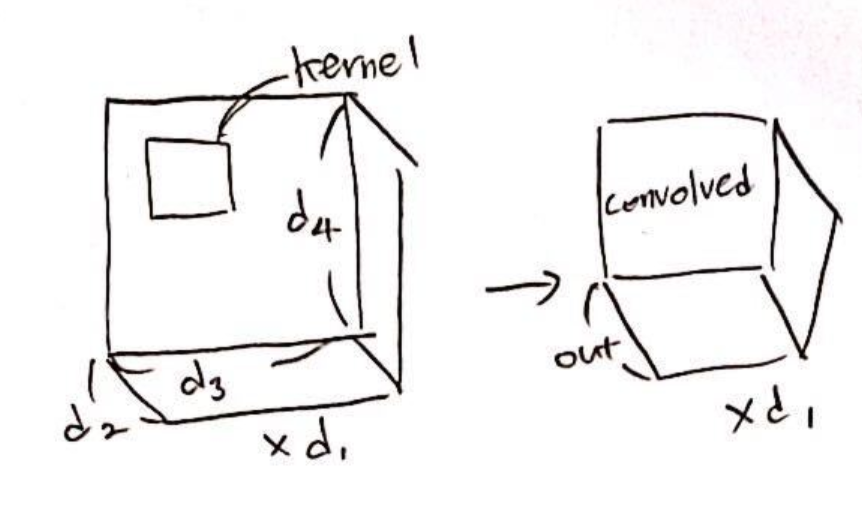
\includegraphics[height=12em]{resources/conv2d.png}
}{
  \begin{itemizec}
    \item $|x| = (d_1, d_2, d_3, d_4)$\bigspace ($rank = 4$)
    \item $d_2 = in\_channels$
    \item $d_3 + 2 \x padding[0] - dilation[0] \x (kernel\_size[0] - 1) - 1 \geq
    0$
    \item $d_4 + 2 \x padding[1] - dilation[1] \x (kernel\_size[1] - 1) - 1 \geq
    0$
    \item $groups | in\_channels$ and $groups | out\_channels$
  \end{itemizec}
}{
  \begin{itemizec}
    \item $|y| = (d_1, out\_channels, h, w)$ where.. refers to the proof tree.
  \end{itemizec}
}{
  \begin{itemizec}
    \item Convolution layer입니다. 선배님의 자료를 \ttt{pytorch}의 사용에 맞게
    풀어 쓴 것입니다.
    \item $kernel\_size$, $stride$와 같은 옵션은 튜플로 구성될 수도 있습니다.
    (가로 세로에 대한 필터크기가 서로 다르도록) 이 경우를 위하여 proof 트리에서
    $kernel\_size[0], [1]$과 같은 표기를 사용하였습니다. 튜플이 아니라 스칼라
    입력인 경우, $kernel\_size[0], [1]$은 모두 $kernel\_size$와 같습니다.
    \item 뒤의 $other\_params..$ 부분은 텐서 shape에 전혀 영향을 주지 않는 인자입니다.
  \end{itemizec}
}
\begin{align*}
  \frac
  {
    \begin{array}{l}
      \sigma \vdash E \Rar e, c \\
      h = \left\lfloor \frac{e[3] + 2 \x padding \ind{0} - dilation \ind{0}
        \x (kernel\_size \ind{0} - 1) - 1}{stride \ind{0}} \right\rfloor + 1 \\
      w = \left\lfloor \frac{e[4] + 2 \x padding \ind{1} - dilation \ind{1}
        \x (kernel\_size \ind{1} - 1) - 1}{stride \ind{1}} \right\rfloor + 1 \\
      e' = (e[1], out, h, w) \\
      c_{dim} = \{ (\op{rank}{e} = 4) \land (e[2] = in) \} \\
      c_h = \{ (e[3] + 2 \x padding[0] - dilation[0] \x (kernel\_size[0] - 1) -
      1 \geq 0) \}\\
      c_w = \{ (e[4] + 2 \x padding[1] - dilation[1] \x (kernel\_size[1] - 1) -
      1 \geq 0) \}\\
      c_{group} = \{ (in \rem groups = 0) \land (out \rem groups = 0) \}
    \end{array}
  }
  {
    \sigma \vdash \module{Conv2d}{in, out, kernel\_size, stride=1, padding=0,
      dilation=1, groups=1}{E} \Rar e', c \cup c_{dim} \cup c_h \cup c_w \cup
      c_{group}
  } \\
  \\
  \text{$kernel\_size, stride, padding, dilation$는 가로-세로별 2-tuple로도 들어갈
  수 있음} \\
  \text{이 경우를 위해 $stride\ind{0}, stride\ind{1}$으로 표기함} \\
  \text{만일 $stride$가 튜플이 아닌 스칼라라면 $stride\ind{0}$ 또는 $\ind{1}$은
    $stride$ 값 자체를 의미}
\end{align*}

\subsection*{(Builtins) \ttt{torch.conv2d}, \ttt{torch.nn.functional.conv2d}}
\prepostc{torch.conv2d(input, weight, bias=None, stride=1, padding=0,
dilation=1, groups=1)}{
  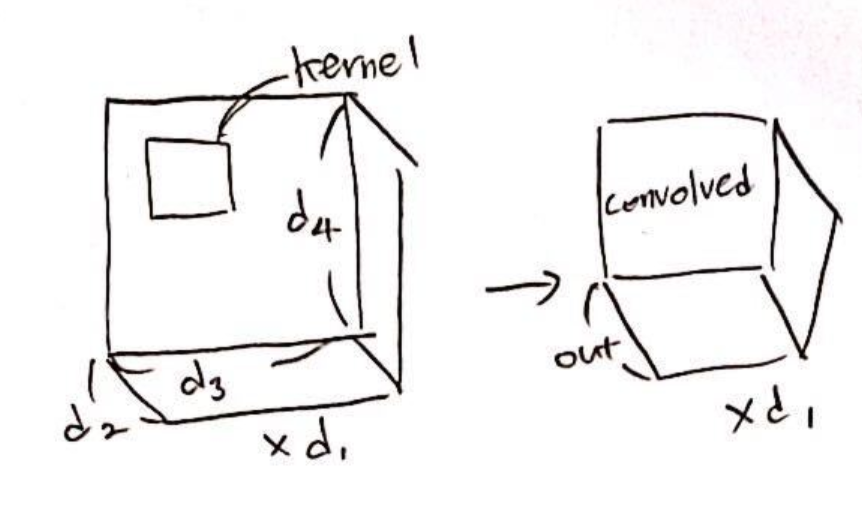
\includegraphics[height=12em]{resources/conv2d.png}
}{
  \begin{itemizec}
    \item $|input| = (batch, in, h_{in}, w_{in})$\bigspace ($rank = 4$)
    \item $|weight| = (out, in\_{group}, h_{weight}, w_{weight})$\bigspace
      ($rank = 4$)
    \item $bias$ is $None$ or $|bias| = (out)$
    \item $h_{weight} + 2 \x padding[0] - dilation[0] \x (h_{weight} - 1) - 1
    \geq 0$
    \item $w_{weight} + 2 \x padding[1] - dilation[1] \x (w_{weight} - 1) - 1
    \geq 0$
    \item $groups | in$, $groups | out$ and $in\_{group} \x group = in$
  \end{itemizec}
}{
  \begin{itemizec}
    \item $|y| = (batch, out, h, w)$ where.. refers to the proof tree.
  \end{itemizec}
}{
  \begin{itemizec}
    \item 컨볼루션 계산을 위해 사용하는 빌트인 함수입니다.
    \item \ttt{torch.conv2d}, \ttt{torch.nn.functional.conv2d} 모두 같은
    방식으로 작동됩니다.
  \end{itemizec}
}
\begin{align*}
  \frac
  {
    \begin{array}{l}
      \sigma \vdash E \Rar e, c \\
      \sigma \vdash F \Rar f, c \\
      \sigma \vdash B \Rar b, c \bigspace \text{if $B$ is not $None$} \\
      (batch, in, h_{in}, w_{in}) = e \\
      (out, in\_group, h_{filter}, w_{filter}) = f \\
      h = \left\lfloor \frac{h_{in} + 2 \x padding \ind{0} - dilation \ind{0}
        \x (h_{filter} - 1) - 1}{stride \ind{0}} \right\rfloor + 1 \\
      w = \left\lfloor \frac{w_{in} + 2 \x padding \ind{1} - dilation \ind{1}
        \x (w_{filter} - 1) - 1}{stride \ind{1}} \right\rfloor + 1 \\
      e' = (batch, out, h, w) \\
      c_{dim} = \{ (\op{rank}{e} = 4) \land (\op{rank}{f} = 4) \} \\
      c_{bias} = \{ ((B = None) \lor (\op{rank}{b} = 1 \land b[1] = out)) \} \\
      c_h = \{ (h_{in} + 2 \x padding[0] - dilation[0] \x (h_{filter} - 1) - 1
        \geq 0) \}\\
      c_w = \{ (w_{in} + 2 \x padding[1] - dilation[1] \x (w_{filter} - 1) - 1
        \geq 0) \}\\
      c_{group} = \{ (in \rem groups = 0) \land (out \rem groups = 0)
        \land (in\_group \x groups = in)\}
    \end{array}
  }
  {
    \sigma \vdash \op{conv2d}{E, F, B=None, stride=1, padding=0,
      dilation=1, groups=1} \Rar e', c \cup c_{dim} \cup c_{bias} \cup c_h \cup
      c_w \cup c_{group}
  } \\
  \\
  \text{$kernel\_size, stride, padding, dilation$는 가로-세로별 2-tuple로도 들어갈
  수 있음} \\
  \text{이 경우를 위해 $stride\ind{0}, stride\ind{1}$으로 표기함} \\
  \text{만일 $stride$가 튜플이 아닌 스칼라라면 $stride\ind{0}$ 또는 $\ind{1}$은
    $stride$ 값 자체를 의미}
\end{align*}

\subsection*{\ttt{torch.nn.Conv1d}}
\prepostc{torch.nn.Conv1d(in\_channels, out\_channels, kernel\_size, stride=1,
padding=0, dilation=1, groups=1, other\_params..)(x)}{
  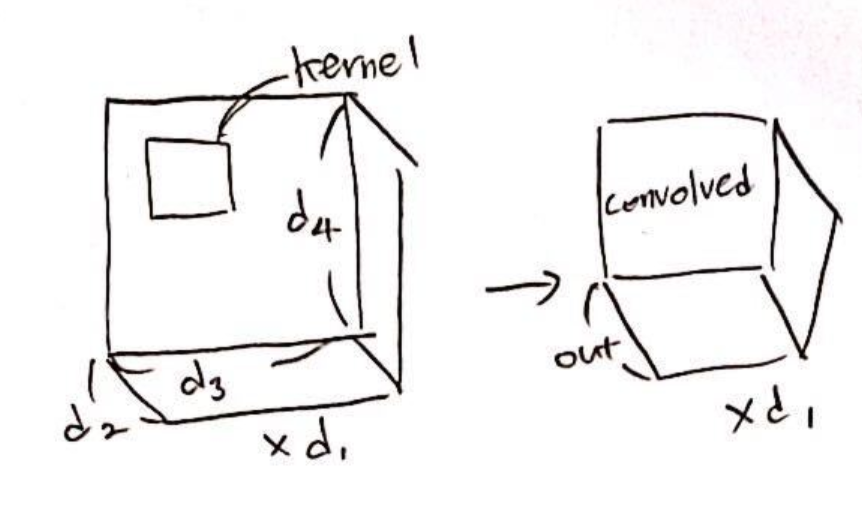
\includegraphics[height=12em]{resources/conv2d.png}
}{
  \begin{itemizec}
    \item $|x| = (d_1, d_2, d_3)$\bigspace ($rank = 3$)
    \item $d_2 = in\_channels$
    \item $d_3 + 2 \x padding - dilation \x (kernel\_size - 1) - 1 \geq
    0$
    \item $groups | in\_channels$ and $groups | out\_channels$
  \end{itemizec}
}{
  \begin{itemizec}
    \item $|y| = (d_1, out\_channels, w)$ where.. refers to the proof tree.
  \end{itemizec}
}{
  \begin{itemizec}
    \item Convolution 1차원 레이어입니다.
    \item $kernel\_size$, $stride$ 등은 1차원 튜플로 구성될 수도 있습니다.
  \end{itemizec}
}
\begin{align*}
  \frac
  {
    \begin{array}{l}
      \sigma \vdash E \Rar e, c \\
      w = \left\lfloor \frac{e[3] + 2 \x padding  - dilation
        \x (kernel\_size - 1) - 1}{stride} \right\rfloor + 1 \\
      e' = (e[1], out, w) \\
      c_{dim} = \{ (\op{rank}{e} = 3) \land (e[2] = in) \} \\
      c_w = \{ (e[3] + 2 \x padding - dilation \x (kernel\_size - 1) - 1 \geq 0) \} \\
      c_{group} = \{ (in \rem groups = 0) \land (out \rem groups = 0) \}
    \end{array}
  }
  {
    \sigma \vdash \module{Conv1d}{in, out, kernel\_size, stride=1, padding=0,
      dilation=1, groups=1}{E} \Rar e', c \cup c_{dim} \cup c_w \cup
      c_{group}
  } \\
  \\
  \text{$kernel\_size, stride, padding, dilation$는 1-length-tuple로 들어올
  수 있음}
\end{align*}

\subsection*{(Builtins) \ttt{torch.conv1d}, \ttt{torch.nn.functional.conv1d}}
\begin{align*}
  \frac
  {
    \begin{array}{l}
      \sigma \vdash E \Rar e, c \\
      \sigma \vdash F \Rar f, c \\
      \sigma \vdash B \Rar b, c \bigspace \text{if $B$ is not $None$} \\
      (batch, in, w_{in}) = e \\
      (out, in\_group, w_{filter}) = f \\
      w = \left\lfloor \frac{w_{in} + 2 \x padding - dilation
        \x (w_{filter} - 1) - 1}{stride} \right\rfloor + 1 \\
      e' = (batch, out, w) \\
      c_{dim} = \{ (\op{rank}{e} = 3) \land (\op{rank}{f} = 3) \} \\
      c_{bias} = \{ ((B = None) \lor (\op{rank}{b} = 1 \land b[1] = out)) \} \\
      c_w = \{ (w_{in} + 2 \x padding - dilation \x (w_{filter} - 1) - 1 \geq 0) \} \\
      c_{group} = \{ (in \rem groups = 0) \land (out \rem groups = 0)
        \land (in\_group \x groups = in)\}
    \end{array}
  }
  {
    \sigma \vdash \op{conv1d}{E, F, B=None, stride=1, padding=0,
      dilation=1, groups=1} \Rar e', c \cup c_{dim} \cup c_{bias} \cup 
      c_w \cup c_{group}
  } \\
  \\
  \text{$kernel\_size, stride, padding, dilation$는 1-length-tuple로 들어올
  수 있음}
\end{align*}

\subsection*{\ttt{torch.nn.Conv3d}}
\begin{align*}
  \frac
  {
    \begin{array}{l}
      \sigma \vdash E \Rar e, c \\
      z = \left\lfloor \frac{e[3] + 2 \x padding \ind{0} - dilation \ind{0}
        \x (kernel\_size \ind{0} - 1) - 1}{stride \ind{0}} \right\rfloor + 1 \\
      h = \left\lfloor \frac{e[4] + 2 \x padding \ind{1} - dilation \ind{1}
        \x (kernel\_size \ind{1} - 1) - 1}{stride \ind{1}} \right\rfloor + 1 \\
      w = \left\lfloor \frac{e[5] + 2 \x padding \ind{2} - dilation \ind{2}
        \x (kernel\_size \ind{2} - 1) - 1}{stride \ind{2}} \right\rfloor + 1 \\
      e' = (e[1], out, z, h, w) \\
      c_{dim} = \{ (\op{rank}{e} = 5) \land (e[2] = in) \} \\
      c_z = \{ (e[3] + 2 \x padding[0] - dilation[0] \x (kernel\_size[0] - 1) -
      1 \geq 0) \}\\
      c_h = \{ (e[4] + 2 \x padding[1] - dilation[1] \x (kernel\_size[1] - 1) -
      1 \geq 0) \}\\
      c_w = \{ (e[5] + 2 \x padding[2] - dilation[2] \x (kernel\_size[2] - 1) -
      1 \geq 0) \}\\
      c_{group} = \{ (in \rem groups = 0) \land (out \rem groups = 0) \}
    \end{array}
  }
  {
    \sigma \vdash \module{Conv3d}{in, out, kernel\_size, stride=1, padding=0,
      dilation=1, groups=1}{E} \Rar e', c \cup c_{dim} \cup c_z \cup c_h \cup
      c_w \cup c_{group}
  } \\
  \\
  \text{$kernel\_size, stride, padding, dilation$는 깊이-가로-세로별 3-tuple로도
  들어갈 수 있음} \\
  \text{이 경우를 위해 $stride\ind{0}, \ind{1}, \ind{2}$으로 표기함} \\
  \text{만일 $stride$가 튜플이 아닌 스칼라라면 $stride\ind{0}, \ind{1}$ 또는 
  $\ind{2}$는 $stride$ 값 자체를 의미}
\end{align*}

\subsection*{(Builtins) \ttt{torch.conv3d}, \ttt{torch.nn.functional.conv3d}}
\begin{align*}
  \frac
  {
    \begin{array}{l}
      \sigma \vdash E \Rar e, c \\
      \sigma \vdash F \Rar f, c \\
      \sigma \vdash B \Rar b, c \bigspace \text{if $B$ is not $None$} \\
      (batch, in, z_{in}, h_{in}, w_{in}) = e \\
      (out, in\_group, z_{filter}, h_{filter}, w_{filter}) = f \\
      z = \left\lfloor \frac{z_{in} + 2 \x padding \ind{0} - dilation \ind{0}
        \x (z_{filter} - 1) - 1}{stride \ind{0}} \right\rfloor + 1 \\
      h = \left\lfloor \frac{h_{in} + 2 \x padding \ind{1} - dilation \ind{1}
        \x (h_{filter} - 1) - 1}{stride \ind{1}} \right\rfloor + 1 \\
      w = \left\lfloor \frac{w_{in} + 2 \x padding \ind{2} - dilation \ind{2}
        \x (w_{filter} - 1) - 1}{stride \ind{2}} \right\rfloor + 1 \\
      e' = (batch, out, z, h, w) \\
      c_{dim} = \{ (\op{rank}{e} = 5) \land (\op{rank}{f} = 5) \} \\
      c_{bias} = \{ ((B = None) \lor (\op{rank}{b} = 1 \land b[1] = out)) \} \\
      c_z = \{ (z_{in} + 2 \x padding[0] - dilation[0] \x (z_{filter} - 1) - 1
        \geq 0) \}\\
      c_h = \{ (h_{in} + 2 \x padding[1] - dilation[1] \x (h_{filter} - 1) - 1
        \geq 0) \}\\
      c_w = \{ (w_{in} + 2 \x padding[2] - dilation[2] \x (w_{filter} - 1) - 1
        \geq 0) \}\\
      c_{group} = \{ (in \rem groups = 0) \land (out \rem groups = 0)
        \land (in\_group \x groups = in)\}
    \end{array}
  }
  {
    \sigma \vdash \op{conv2d}{E, F, B=None, stride=1, padding=0,
      dilation=1, groups=1} \Rar e', c \cup c_{dim} \cup c_{bias} \cup c_z 
        \cup c_h \cup c_w \cup c_{group}
  } \\
  \\
  \text{$kernel\_size, stride, padding, dilation$는 가로-세로별 3-tuple로도 들어갈
  수 있음} \\
  \text{이 경우를 위해 $stride\ind{0}, \ind{1}, \ind{2}$으로 표기함} \\
  \text{만일 $stride$가 튜플이 아닌 스칼라라면 $stride\ind{0}, \ind{1}$ 또는 
  $\ind{2}$는 $stride$ 값 자체를 의미}
\end{align*}

\subsection*{\ttt{torch.nn.ConvTranspose1d}}
\prepostc{torch.nn.ConvTranspose1d(in\_channels, out\_channels, kernel\_size,
stride=1, padding=0, output\_padding=0, groups=1, bias=True, dilation=1,
padding\_mode=`zeros')(x)}{
  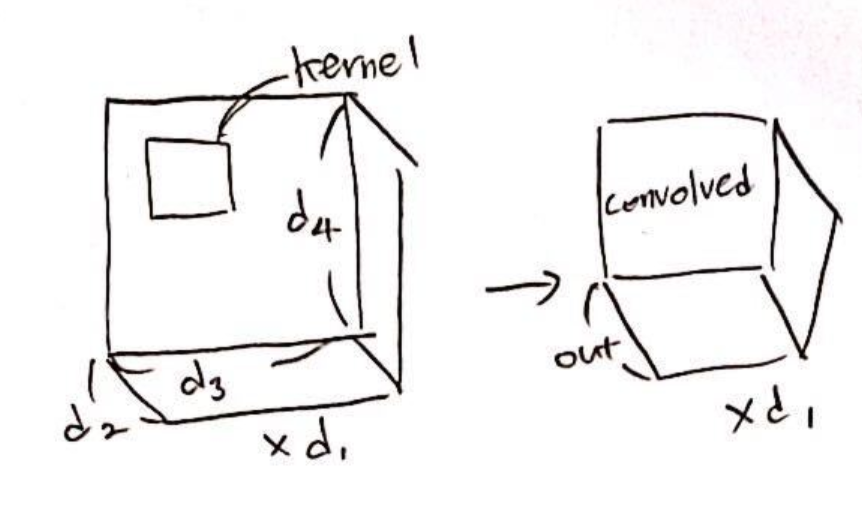
\includegraphics[height=12em]{resources/conv2d.png}
}{
  \begin{itemizec}
    \item $|x| = (d_1, d_2, d_3)$\bigspace ($rank = 3$)
    \item $d_2 = in\_channels$
    \item $kernel\_size \leq d_3 + 2 \x padding$
    \item $groups | in\_channels$ and $groups | out\_channels$
  \end{itemizec}
}{
  \begin{itemizec}
    \item $|y| = (d_1, out\_channels, w)$ where.. refers to the proof tree.
  \end{itemizec}
}{
  \begin{itemizec}
    \item Convolution에서 gradient를 구하기위한 레이어로 보시면 됩니다.
    \item $kernel\_size$, $stride$ 등은 1차원 튜플로 구성될 수도 있습니다.
    \item \texttt{bias}, \texttt{pad\_mode} 옵션은 shape에 영향을 주지 않습니다.
  \end{itemizec}
}
\begin{align*}
  \frac
  {
    \begin{array}{l}
      \sigma \vdash E \Rar e, c \\
      w = (e[3] - 1) \x stride - 2 \x pad + dilation \x (kernel - 1) + out\_pad
      + 1\\
      e' = (e[1], out, w) \\
      c_{dim} = \{ (\op{rank}{e} = 3) \land (e[2] = in) \land (w > 0) \} \\
      c_{group} = \{ (in \rem groups = 0) \land (out \rem groups = 0) \}
    \end{array}
  }
  {
    \begin{array}{ll}
      \sigma \vdash & \module{ConvTranspose1d}{in, out, kernel, stride=1, pad=0,
        out\_pad=0, groups=1, bias=True, dilation=1, pad\_mode}{E} \\
      & \Rar e', c \cup c_{dim} \cup c_{group}
    \end{array}
  } \\
  \\
  \text{$kernel\_size, stride, padding, dilation$는 1-length-tuple로 들어올
  수 있음}
\end{align*}

\subsection*{(Builtins) \ttt{torch.conv\_transpose1d}, \ttt{torch.nn.functional.conv\_transpose1d}}
\begin{align*}
  \frac
  {
    \begin{array}{l}
      \sigma \vdash E \Rar e, c_e \\
      \sigma \vdash F \Rar f, c_f \\
      \sigma \vdash B \Rar b, c_b \bigspace \text{if $B$ is not $None$} \\
      w = (e[3] - 1) \x stride - 2 \x pad + dilation \x (f[3] - 1) + out\_pad
      + 1\\
      e' = (e[1], f[2] \x groups, w) \\
      c_{dim} = \{ (\op{rank}{e} = 3) \land (\op{rank}{f} = 3) \land (f[1] = e[2])
        \land (w > 0) \} \\
      c_{bias} = \{ (B = None \lor b = (f[2] \x groups) ) \} \\
      c_{group} = \{ (in \rem groups = 0) \}
    \end{array}
  }
  {
    \begin{array}{ll}
      \sigma \vdash & \op{conv\_transpose1d}{E, F, B=None, stride=1, pad=0,
        out\_pad=0, groups=1, dilation=1} \\
      & \Rar e', c \cup c_{dim} \cup c_{bias} \cup c_{group}
    \end{array}
  } \\
  \\
  \text{$kernel\_size, stride, padding, dilation$는 1-length-tuple로 들어올
  수 있음}
\end{align*}

\section*{Activations}
\subsection*{\texttt{torch.nn.MaxPool2d}}
\prepostc{torch.nn.MaxPool2d(kernel\_size, stride=kernel\_size,
padding=0, dilation=1)(x)}{
  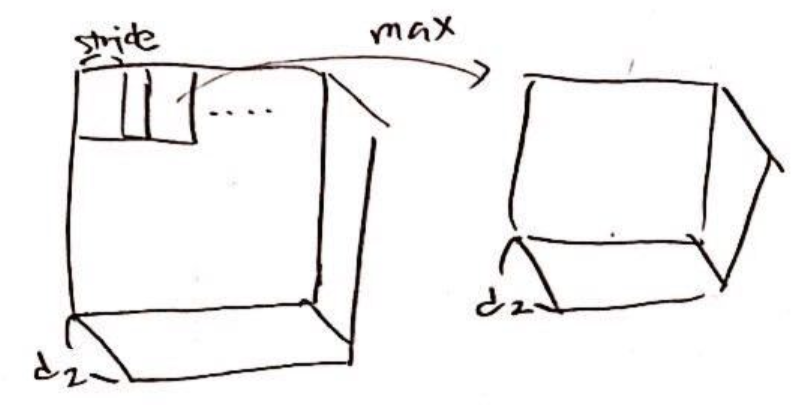
\includegraphics[height=10em]{resources/maxpool2d.png}
}{
  \begin{itemizec}
    \item $|x| = (d_1, d_2, d_3, d_4)\text{ or } (d_2, d_3, d_4)$
    \item $d_3 + 2 \x padding \ind{0} - dilation \ind{0}
        \x (kernel\_size \ind{0} - 1) - 1 \geq 0 $
    \item $d_4 + 2 \x padding \ind{1} - dilation \ind{1}
        \x (kernel\_size \ind{1} - 1) - 1 \geq 0 $
  \end{itemizec}
}{
  \begin{itemizec}
    \item $(d_1, d_2, h, w) \text{ or } (d_2, h, w)$ where.. proof tree.
  \end{itemizec}
}{
  \begin{itemizec}
    \item Convolution 다음 activation으로 자주 쓰이는 MaxPool 레이어 입니다.
  \end{itemizec}
}
\begin{align*}
  \frac
  {
    \begin{array}{l}
      \sigma \vdash E \Rar e, c \\
      k = \op{rank}{e} \\
      h_{orig} = e[k-1] \\
      w_{orig} = e[k] \\
      h = \left\lfloor \frac{h_{orig} + 2 \x padding \ind{0} - dilation \ind{0}
        \x (kernel\_size \ind{0} - 1) - 1}{stride \ind{0}} \right\rfloor + 1 \\
      w = \left\lfloor \frac{w_{orig} + 2 \x padding \ind{1} - dilation \ind{1}
        \x (kernel\_size \ind{1} - 1) - 1}{stride \ind{1}} \right\rfloor + 1 \\
      e' = e\indr{1}{k-2} \conc (h, w) \\
      c_{dim} = \{ (k = 3 \lor k = 4) \} \\
      c_h = \{ (h_{orig} + 2 \x padding \ind{0} - dilation \ind{0}
        \x (kernel\_size \ind{0} - 1) - 1 \geq 0) \} \\
      c_w = \{ (w_{orig} + 2 \x padding \ind{1} - dilation \ind{1}
        \x (kernel\_size \ind{1} - 1) - 1 \geq 0) \} \\
    \end{array}
  }
  {
    \begin{array}{c}
      \sigma \vdash \module{MaxPool2d}{kernel\_size, stride=kernel\_size,
        padding=0, dilation=1}{E}
        \Rar e', c \cup c_{dim} \cup c_w \cup c_h 
    \end{array}
  } \\
  \\
  \text{$kernel\_size, stride, padding, dilation$는 가로-세로별 2-tuple로도 들어갈
  수 있음} \\
  \text{이 경우를 위해 $stride\ind{0}, stride\ind{1}$으로 표기함} \\
  \text{만일 $stride$가 튜플이 아닌 스칼라라면 $stride\ind{0}$ 또는 $\ind{1}$은
    $stride$ 값 자체를 의미}
\end{align*}

\prepost{torch.nn.MaxPool2d(kernel\_size, stride=..., dilation=1,
return\_indices=False, ceil\_mode=False)(x)}{
  
\includegraphics[height=8em]{resources/maxpool2d_ri.png}
}{
  \begin{itemizec}
    \item $|x| = (d_1, d_2, d_3, d_4)\text{ or } (d_2, d_3, d_4)$
    \item $d_3 + 2 \x padding \ind{0} - dilation \ind{0}
        \x (kernel\_size \ind{0} - 1) - 1 \geq 0 $
    \item $d_4 + 2 \x padding \ind{1} - dilation \ind{1}
        \x (kernel\_size \ind{1} - 1) - 1 \geq 0 $
  \end{itemizec}
}{
  \begin{itemizec}
    \item $(d_1, d_2, h, w) \text{ or } (d_2, h, w)$ where.. proof tree.
    \item $return\_indices$가 $True$이면 인덱스 번호까지 튜플로 반환
    \item $ceil\_mode$가 $True$이면 $floor$대신 $ceil$로 shape 계산
  \end{itemizec}
}
\begin{align*}
  \frac
  {
    \begin{array}{l}
      \sigma \vdash E \Rar e, c \\
      k = \op{rank}{e} \\
      h_{orig} = e[k-1] \\
      w_{orig} = e[k] \\
      h = \left\lfloor \frac{h_{orig} + 2 \x padding \ind{0} - dilation \ind{0}
        \x (kernel\_size \ind{0} - 1) - 1}{stride \ind{0}} \right\rfloor + 1 \\
      w = \left\lfloor \frac{w_{orig} + 2 \x padding \ind{1} - dilation \ind{1}
        \x (kernel\_size \ind{1} - 1) - 1}{stride \ind{1}} \right\rfloor + 1 \\
      h_{ceil} = \left\lceil \frac{h_{orig} + 2 \x padding \ind{0} - dilation \ind{0}
        \x (kernel\_size \ind{0} - 1) - 1}{stride \ind{0}} \right\rceil + 1 \\
      w_{ceil} = \left\lceil \frac{w_{orig} + 2 \x padding \ind{1} - dilation \ind{1}
        \x (kernel\_size \ind{1} - 1) - 1}{stride \ind{1}} \right\rceil + 1 \\
      e' = \ifs{ceil\_mode}{e\indr{1}{k-2} \conc (h_{ceil},
      w_{ceil})}{e\indr{1}{k-2} \conc (h, w)} \\
      e_{out} = \ifs{return\_indices}{(e', e')}{e'}\\
      c_{dim} = \{ (k = 3 \lor k = 4) \} \\
      c_h = \{ (h_{orig} + 2 \x padding \ind{0} - dilation \ind{0}
        \x (kernel\_size \ind{0} - 1) - 1 \geq 0) \} \\
      c_w = \{ (w_{orig} + 2 \x padding \ind{1} - dilation \ind{1}
        \x (kernel\_size \ind{1} - 1) - 1 \geq 0) \} \\
    \end{array}
  }
  {
    \begin{array}{rl}
      \sigma \vdash & \module{MaxPool2d}{kernel\_size, stride, padding,
        dilation, return\_indices, ceil\_mode}{E} \\
      & \Rar e', c \cup c_{dim} \cup c_w \cup c_h 
    \end{array}
  } \\
  \\
  \text{$return\_indices$가 $True$이면 (결과, 인덱스) 튜플 형태로 반환}\\
  \text{$ceil\_mode$가 $True$이면 $floor$대신 $ceil$함수로 계산}
\end{align*}

\begin{align*}
  \frac
  {
    \begin{array}{l}
      \sigma \vdash \op{torch.nn.MaxPool2d}{E, other\_params...} \Rar e, c \\
    \end{array}
  }
  {
    \sigma \vdash \op{max\_pool2d}{E, other\_params...} \Rar e, c
  } \\
  \\
  \text{(Builtins) \ttt{torch.max\_pool2d}나
  \ttt{torch.nn.functional.max\_pool2d}에 대한 적용}
\end{align*}

\subsection*{(Builtins) \texttt{torch.max\_pool2d},
\texttt{torch.nn.functional.max\_pool2d}}
\prepostc{torch.max\_pool2d(input, kernel\_size, stride=kernel\_size,
padding=0, dilation=1, ceil\_mode=False)}{
  %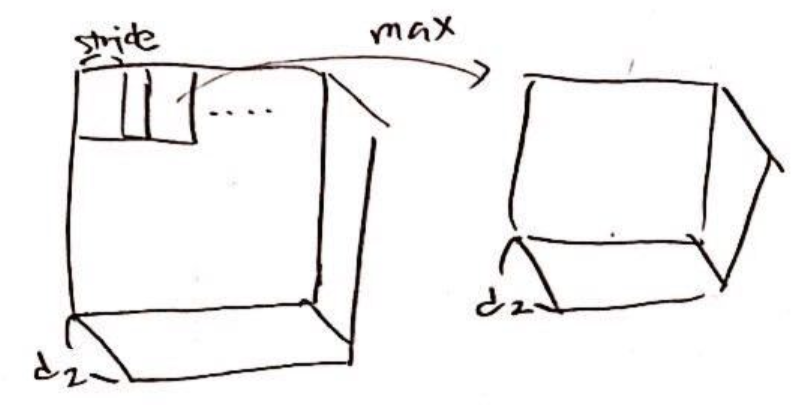
\includegraphics[height=10em]{resources/maxpool2d.png}
}{
  \begin{itemizec}
    \item $|input| = (d_1, d_2, d_3, d_4)\text{ or } (d_2, d_3, d_4)$
    \item $d_3 + 2 \x padding \ind{0} - dilation \ind{0}
        \x (kernel\_size \ind{0} - 1) - 1 \geq 0 $
    \item $d_4 + 2 \x padding \ind{1} - dilation \ind{1}
        \x (kernel\_size \ind{1} - 1) - 1 \geq 0 $
  \end{itemizec}
}{
  \begin{itemizec}
    \item $(d_1, d_2, h, w) \text{ or } (d_2, h, w)$ where.. proof tree.
  \end{itemizec}
}{
  \begin{itemizec}
    \item $\mtt{torch.max\_pool2d} \equiv \mtt{torch.nn.functional.max\_pool2d}$
    \item Builtin 함수인데, 특이한 점은 \texttt{return\_indices} parameter가
    없다는 것입니다. (\texttt{max\_pool2d\_with\_indices}라는 다른 함수로
    분리되어있습니다.)
  \end{itemizec}
}
\begin{align*}
  \frac
  {
    \begin{array}{ll}
      \sigma \vdash E \Rar e, c \\
      k = \op{rank}{e} \\
      h_{orig} = e[k-1] \\
      w_{orig} = e[k] \\
      h = \left\lfloor \frac{h_{orig} + 2 \x padding \ind{0} - dilation \ind{0}
        \x (kernel\_size \ind{0} - 1) - 1}{stride \ind{0}} \right\rfloor + 1 &
        \text{(if $ceil\_mode$ is $True$, then use $\lceil \cdot \rceil$)}\\
      w = \left\lfloor \frac{w_{orig} + 2 \x padding \ind{1} - dilation \ind{1}
        \x (kernel\_size \ind{1} - 1) - 1}{stride \ind{1}} \right\rfloor + 1 &
        \text{(if $ceil\_mode$ is $True$, then use $\lceil \cdot \rceil$)}\\
      e' = e\indr{1}{k-2} \conc (h, w) \\
      c_{dim} = \{ (k = 3 \lor k = 4) \} \\
      c_h = \{ (h_{orig} + 2 \x padding \ind{0} - dilation \ind{0}
        \x (kernel\_size \ind{0} - 1) - 1 \geq 0) \} \\
      c_w = \{ (w_{orig} + 2 \x padding \ind{1} - dilation \ind{1}
        \x (kernel\_size \ind{1} - 1) - 1 \geq 0) \} \\
    \end{array}
  }
  {
    \begin{array}{c}
      \sigma \vdash \op{max\_pool2d}{E, kernel\_size, stride=kernel\_size,
        padding=0, dilation=1}
        \Rar e', c \cup c_{dim} \cup c_w \cup c_h 
    \end{array}
  } \\
  \\
  \text{$kernel\_size, stride, padding, dilation$는 가로-세로별 2-tuple로도 들어갈
  수 있음} \\
  \text{이 경우를 위해 $stride\ind{0}, stride\ind{1}$으로 표기함} \\
  \text{만일 $stride$가 튜플이 아닌 스칼라라면 $stride\ind{0}$ 또는 $\ind{1}$은
    $stride$ 값 자체를 의미}
\end{align*}

\prepostc{torch.nn.functional.max\_pool2d\_with\_indices(input, kernel\_size,
stride=..., dilation=1, ceil\_mode=False)}{
  
\includegraphics[height=8em]{resources/maxpool2d_ri.png}
}{
  \begin{itemizec}
    \item $|x| = (d_1, d_2, d_3, d_4)\text{ or } (d_2, d_3, d_4)$
    \item $kernel\_size[0] \leq d_3 + 2 \x padding[0]$
    \item $kernel\_size[1] \leq d_4 + 2 \x padding[1]$
  \end{itemizec}
}{
  \begin{itemizec}
    \item 2-tuple of $(d_1, d_2, h, w) \text{ or } (d_2, h, w)$ where.. proof tree.
  \end{itemizec}
}{
  \begin{itemizec}
    \item \texttt{torch.}에는 없고, \texttt{torch.nn.functional}에만 있습니다.
  \end{itemizec}
}
\begin{align*}
  \frac
  {
    \begin{array}{ll}
      \sigma \vdash E \Rar e, c \\
      k = \op{rank}{e} \\
      h_{orig} = e[k-1] \\
      w_{orig} = e[k] \\
      h = \left\lfloor \frac{h_{orig} + 2 \x padding \ind{0} - dilation \ind{0}
        \x (kernel\_size \ind{0} - 1) - 1}{stride \ind{0}} \right\rfloor + 1 &
        \text{(if $ceil\_mode$ is $True$, then use $\lceil \cdot \rceil$)}\\
      w = \left\lfloor \frac{w_{orig} + 2 \x padding \ind{1} - dilation \ind{1}
        \x (kernel\_size \ind{1} - 1) - 1}{stride \ind{1}} \right\rfloor + 1 &
        \text{(if $ceil\_mode$ is $True$, then use $\lceil \cdot \rceil$)}\\
      e' = e\indr{1}{k-2} \conc (h, w) \\
      c_{dim} = \{ (k = 3 \lor k = 4) \} \\
      c_h = \{ (h_{orig} + 2 \x padding \ind{0} - dilation \ind{0}
        \x (kernel\_size \ind{0} - 1) - 1 \geq 0) \} \\
      c_w = \{ (w_{orig} + 2 \x padding \ind{1} - dilation \ind{1}
        \x (kernel\_size \ind{1} - 1) - 1 \geq 0) \} \\
    \end{array}
  }
  {
    \begin{array}{rl}
      \sigma \vdash & \op{max\_pool2d\_with\_indices}{E, kernel\_size, stride, padding,
        dilation, ceil\_mode} \\
      & \Rar (e', e'), c \cup c_{dim} \cup c_w \cup c_h 
    \end{array}
  }
\end{align*}

\subsection*{\texttt{torch.nn.AvgPool2d}}
\prepostc{torch.nn.AvgPool2d(kernel\_size, stride=kernel\_size,
padding=0, other\_params, ...)(x)}{
  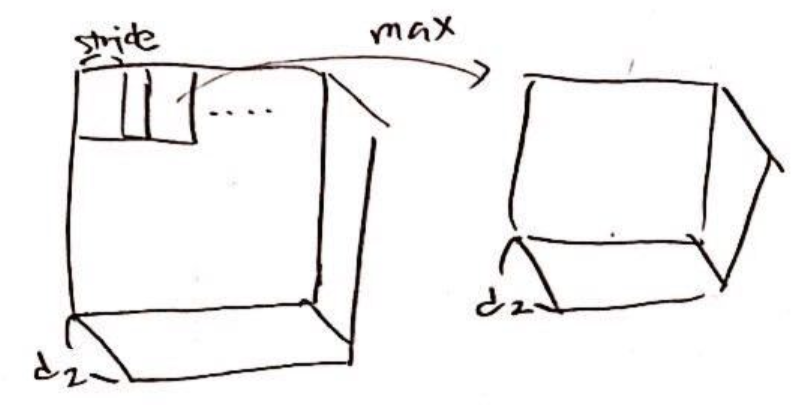
\includegraphics[height=10em]{resources/maxpool2d.png}
}{
  \begin{itemizec}
    \item $|x| = (d_1, d_2, d_3, d_4)\text{ or } (d_2, d_3, d_4)$
    \item $kernel\_size[0] \leq d_3 + 2 \x padding[0]$
    \item $kernel\_size[1] \leq d_4 + 2 \x padding[1]$
  \end{itemizec}
}{
  \begin{itemizec}
    \item $(d_1, d_2, h, w) \text{ or } (d_2, h, w)$ where.. proof tree.
  \end{itemizec}
}{
  \begin{itemizec}
    \item 셀들의 평균으로 정규화하는 레이어
    \item \texttt{MaxPool2d}와 비슷하나 $dilation$과 $return\_indices$ 옵션이
    없음
  \end{itemizec}
}
\begin{align*}
  \frac
  {
    \begin{array}{ll}
      \sigma \vdash E \Rar e, c \\
      k = \op{rank}{e} \\
      h_{orig} = e[k-1] \\
      w_{orig} = e[k] \\
      h = \left\lfloor \frac{h_{orig} + 2 \x padding \ind{0} - 
        kernel\_size \ind{0}}{stride \ind{0}} \right\rfloor + 1 &
        \text{(if $ceil\_mode$ is $True$, then use $\lceil \cdot \rceil$)}\\
      w = \left\lfloor \frac{w_{orig} + 2 \x padding \ind{1} -
        kernel\_size \ind{1}}{stride \ind{1}} \right\rfloor + 1 &
        \text{(if $ceil\_mode$ is $True$, then use $\lceil \cdot \rceil$)}\\
      e' = e\indr{1}{k-2} \conc (h, w) \\
      c_{dim} = \{ (k = 3 \lor k = 4) \} \\
      c_w = \{ (kernel\_size\ind{0} \leq h_{orig} + 2 \x padding \ind{0}) \} \\
      c_h = \{ (kernel\_size\ind{1} \leq w_{orig} + 2 \x padding \ind{1}) \} 
    \end{array}
  }
  {
    \begin{array}{c}
      \sigma \vdash \module{MaxPool2d}{kernel\_size, stride=kernel\_size,
        padding=0, other\_params, ...}{E}
        \Rar e', c \cup c_{dim} \cup c_w \cup c_h 
    \end{array}
  } \\
  \\
  \text{$kernel\_size, stride, padding$는 가로-세로별 2-tuple로도 들어갈
  수 있음} \\
  \text{이 경우를 위해 $stride\ind{0}, stride\ind{1}$으로 표기함} \\
  \text{만일 $stride$가 튜플이 아닌 스칼라라면 $stride\ind{0}$ 또는 $\ind{1}$은
    $stride$ 값 자체를 의미}
\end{align*}

\subsection*{\texttt{torch.nn.AdaptiveAvgPool2d}}
\prepostc{torch.nn.AdaptiveAvgPool2d(output\_size)(x)}{
  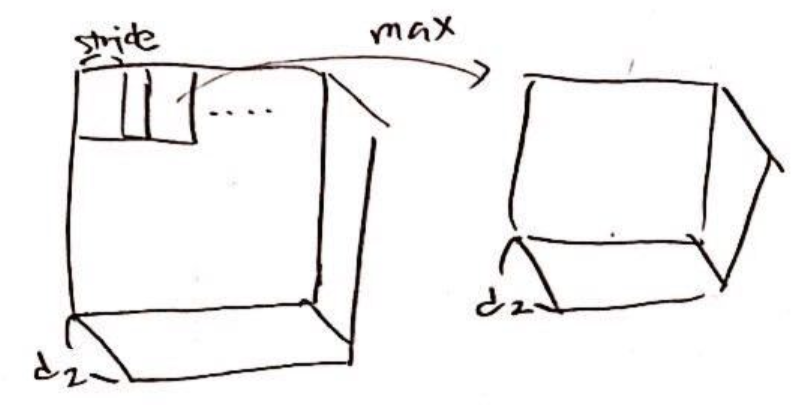
\includegraphics[height=10em]{resources/maxpool2d.png}
}{
  \begin{itemizec}
    \item $|x| = (d_1, d_2, d_3, d_4)\text{ or } (d_2, d_3, d_4)$
    \begin{itemize}
      \item $\op{rank}{|x|} = 3$ or $4$
    \end{itemize}
  \end{itemizec}
}{
  \begin{itemizec}
    \item $(d_1, d_2, output\_size[0], output\_size[1])$ \bigspace
    $\text{or } (d_2, output\_size[0], output\_size[1])$
  \end{itemizec}
}{
  \begin{itemizec}
    \item 출력 shape를 강제하는 평균 pool 입니다.
    \item $output\_size$는 2-tuple이 될 수도 있습니다.
    \item $output\_size > d_3 \text{ or } d_4$인 상황에도 오류없이 작동합니다.
  \end{itemizec}
}
\begin{align*}
  \frac
  {
    \begin{array}{l}
      \sigma \vdash E \Rar e, c \\
      k = \op{rank}{e} \\
      e' = e\indr{1}{k-2} \conc (output\_size[0], output\_size[1]) \\
      c_{dim} = \{ (k = 3 \lor k = 4) \} \\
    \end{array}
  }
  {
    \begin{array}{c}
      \sigma \vdash \module{AdaptiveAvgPool2d}{output\_size}{E}
        \Rar e', c \cup c_{dim} \cup c_w \cup c_h 
    \end{array}
  } \\
  \\
  \text{$output\_size$는 가로-세로별 2-tuple로도 들어갈
  수 있음} \\
  \text{이 경우를 위해 $output\_size\ind{0}, output\_size\ind{1}$으로 표기함} \\
  \text{만일 $output\_size$가 튜플이 아닌 스칼라라면 $output\_size\ind{0}$ 또는 $\ind{1}$은
    $output\_size$ 값 자체를 의미}
\end{align*}

\subsection*{\texttt{torch.nn.AdaptiveAvgPool3d}}
\prepostc{torch.nn.AdaptiveAvgPool3d(output\_size)(x)}{
  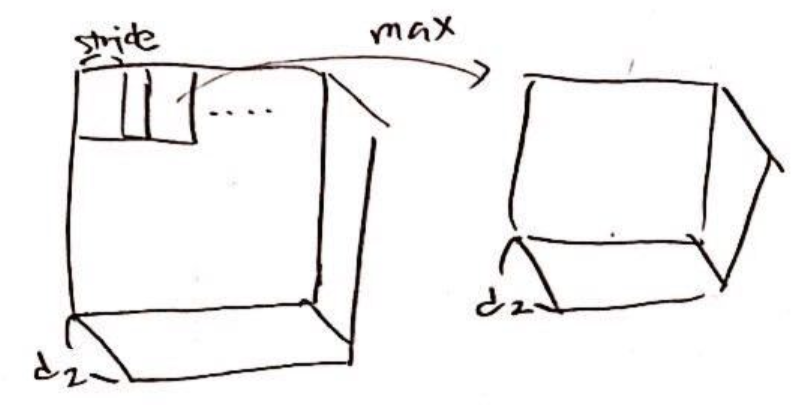
\includegraphics[height=10em]{resources/maxpool2d.png}
}{
  \begin{itemizec}
    \item $|x| = (d_1, d_2, d_3, d_4, d_5)\text{ or } (d_2, d_3, d_4, d_5)$
    \begin{itemize}
      \item $\op{rank}{|x|} = 4$ or $5$
    \end{itemize}
  \end{itemizec}
}{
  \begin{itemizec}
    \item $(d_1, d_2, d_3, output\_size[0], output\_size[1])$ \bigspace
    $\text{or } (d_2, d_3, output\_size[0], output\_size[1])$
  \end{itemizec}
}{
  \begin{itemizec}
    \item 출력 shape를 강제하는 평균 pool 입니다.
    \item $output\_size$는 3-tuple이 될 수도 있습니다.
    \item $output\_size > d_3, d_4 \text{ or } d_5$인 상황에도 오류없이 작동합니다.
  \end{itemizec}
}
\begin{align*}
  \frac
  {
    \begin{array}{l}
      \sigma \vdash E \Rar e, c \\
      k = \op{rank}{e} \\
      e' = e\indr{1}{k-2} \conc (output\_size[0], output\_size[1]) \\
      c_{dim} = \{ (k = 4 \lor k = 5) \} \\
    \end{array}
  }
  {
    \begin{array}{c}
      \sigma \vdash \module{AdaptiveAvgPool3d}{output\_size}{E}
        \Rar e', c \cup c_{dim} \cup c_w \cup c_h 
    \end{array}
  } \\
  \\
  \text{$output\_size$는 깊이-가로-세로별 3-tuple로도 들어갈
  수 있음} \\
  \text{이 경우를 위해 $output\_size\ind{0}, \ind{1} \ind{2}$으로 표기함} \\
  \text{만일 $output\_size$가 튜플이 아닌 스칼라라면 $output\_size\ind{0},
  \ind{1}$ 또는 $\ind{2}$은 $output\_size$ 값 자체를 의미}
\end{align*}


\section*{Normalizations}
\subsection*{\texttt{torch.nn.BatchNorm2d}}
\prepost{torch.nn.BatchNorm2d(num\_features, other\_params...)(x)}{
  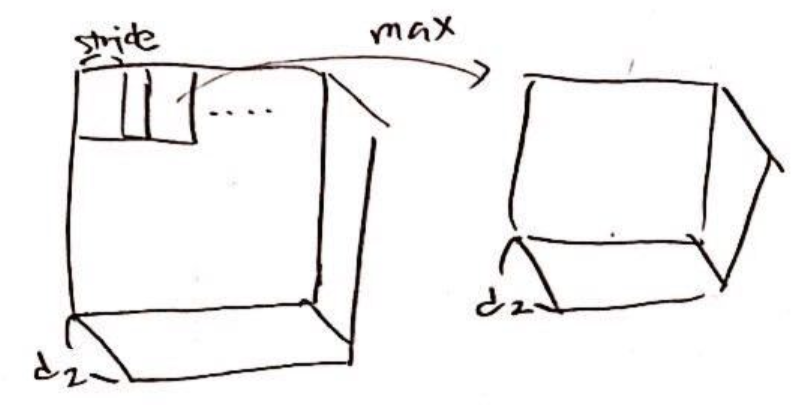
\includegraphics[height=10em]{resources/maxpool2d.png}
}{
  \begin{itemizec}
    \item $|x| = (d_1, d_2, d_3, d_4)$\bigspace ($\mtt{rank} = 4$)
    \item $d_2 = num\_features$
  \end{itemizec}
}{
  \begin{itemizec}
    \item $|y| = (d_1, d_2, d_3, d_4)$\bigspace (same shape to $x$)
  \end{itemizec}
}
\begin{align*}
  \frac
  {
    \begin{array}{l}
      \sigma \vdash E \Rar e, c \\
      c' = \{ (\op{rank}{e} = 4) \land (e[2] = num\_features) \}
    \end{array}
  }
  {
    \sigma \vdash \module{BatchNorm2d}{num\_features, other\_params}{E} \Rar e,
      c \cup c'
  }
\end{align*}


\subsection*{\texttt{torch.nn.BatchNorm3d}}
\prepost{torch.nn.BatchNorm3d(num\_features, other\_params...)(x)}{
  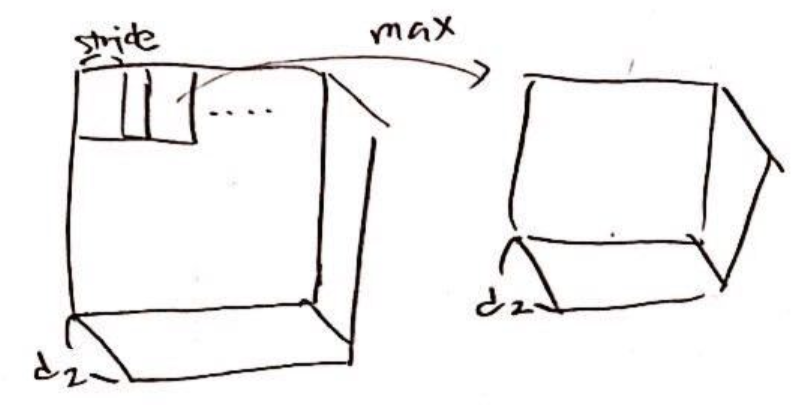
\includegraphics[height=10em]{resources/maxpool2d.png}
}{
  \begin{itemizec}
    \item $|x| = (d_1, d_2, d_3, d_4, d_5)$\bigspace ($\mtt{rank} = 5$)
    \item $d_2 = num\_features$
  \end{itemizec}
}{
  \begin{itemizec}
    \item $|y| = (d_1, d_2, d_3, d_4, d_5)$\bigspace (same shape to $x$)
  \end{itemizec}
}
\begin{align*}
  \frac
  {
    \begin{array}{l}
      \sigma \vdash E \Rar e, c \\
      c' = \{ (\op{rank}{e} = 5) \land (e[2] = num\_features) \}
    \end{array}
  }
  {
    \sigma \vdash \module{BatchNorm3d}{num\_features, other\_params}{E} \Rar e,
      c \cup c'
  }
\end{align*}


\subsection*{\texttt{torch.nn.BatchNorm1d}}
\prepost{torch.nn.BatchNorm1d(num\_features, other\_params...)(x)}{
  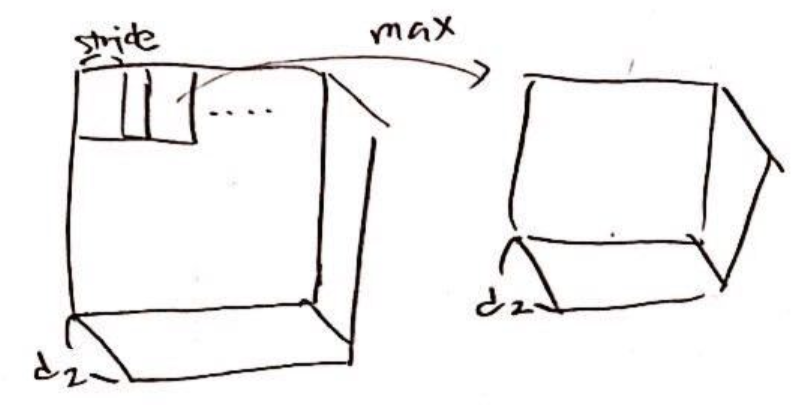
\includegraphics[height=10em]{resources/maxpool2d.png}
}{
  \begin{itemizec}
    \item $|x| = (d_1, d_2, d_3)$\bigspace ($\mtt{rank} = 3$)
    \item $d_2 = num\_features$
  \end{itemizec}
}{
  \begin{itemizec}
    \item $|y| = (d_1, d_2, d_3)$\bigspace (same shape to $x$)
  \end{itemizec}
}
\begin{align*}
  \frac
  {
    \begin{array}{l}
      \sigma \vdash E \Rar e, c \\
      c' = \{ (\op{rank}{e} = 3) \land (e[2] = num\_features) \}
    \end{array}
  }
  {
    \sigma \vdash \module{BatchNorm1d}{num\_features, other\_params}{E} \Rar e,
      c \cup c'
  }
\end{align*}


\subsection*{(Builtins) \texttt{torch.batch\_norm},
\texttt{torch.nn.functional.batch\_norm}}
\prepostc{torch.batch\_norm(input, running\_mean, running\_var, weight=None,
bias=None, training=False, other\_params,...)(x)}{
  %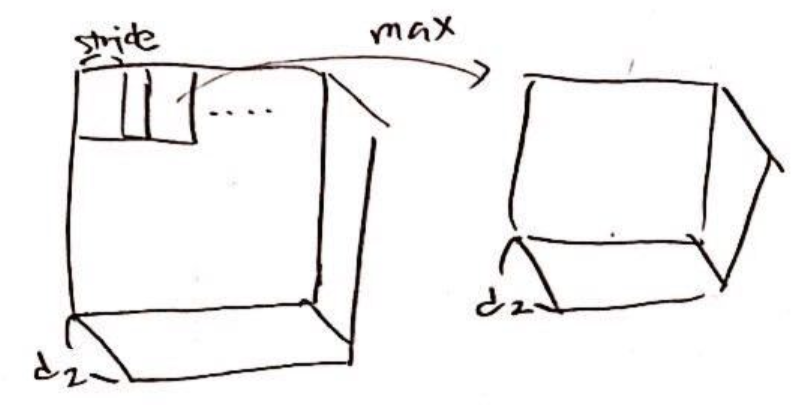
\includegraphics[height=10em]{resources/maxpool2d.png}
}{
  \begin{itemizec}
    \item $|input| = (d_1, d_2, d_3, \dots, d_k)$
    \item $k \geq 2$
    \item If $training$ is $False$ then
    \begin{itemize}
      \item $|running\_mean| = |running\_var| = (d_2)$
    \end{itemize}
    Otherwise,
    \begin{itemize}
      \item $running\_mean$ is $None$ or $|running\_mean| = (d_2)$ (also for $running\_var$)
    \end{itemize}
    \item $weight$ is $None$ or $|weight| = (d_2)$ (also for $bias$)
  \end{itemizec}
}{
  \begin{itemizec}
    \item $|y| = (d_1, d_2, d_3, \dots, d_k) = |x|$
  \end{itemizec}
}{
  \begin{itemizec}
    \item \texttt{BatchNormNd}를 사용하기 위한 일반화된 함수입니다.
  \end{itemizec}
}
\begin{align*}
  \frac
  {
    \begin{array}{rl}
      \sigma \vdash E \Rar e, c_e \\
      \sigma \vdash M \Rar m, c_m & \text{if $M$ is not $None$} \\
      \sigma \vdash V \Rar v, c_v & \text{if $V$ is not $None$} \\
      \sigma \vdash W \Rar w, c_w & \text{if $W$ is not $None$} \\
      \sigma \vdash B \Rar b, c_b & \text{if $B$ is not $None$} \\
      c_{rank} = \{ (\op{rank}{e} \geq 2) \} \\
      c_{m}' = \{ ((training=True \land M = None) \lor (m = (d_2)) \}\\
      c_{v}' = \{ ((training=True \land V = None) \lor (v = (d_2)) \}\\
      c_{w}' = \{ ((W = None) \lor (w = (d_2)) \}\\
      c_{b}' = \{ ((B = None) \lor (b = (d_2)) \}
    \end{array}
  }
  {
    \sigma \vdash \op{batch\_norm}{E, M, V, W, B, training, other\_params,...} \Rar e,
      c_e \cup c_m \cup \cdots \cup c_b \cup c_{rank} \cup c_m' \cup \cdots \cup
      c_b'
  }
\end{align*}


\subsection*{\texttt{torch.nn.GroupNorm}}
\prepost{torch.nn.GroupNorm(num\_groups, num\_channels, other\_params, ...)(x)}{
  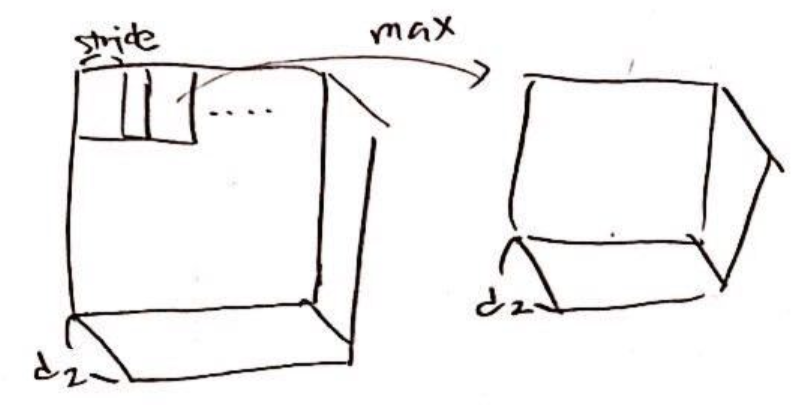
\includegraphics[height=10em]{resources/maxpool2d.png}
}{
  \begin{itemizec}
    \item $|x| = (d_1, d_2, \dots, d_k)$
    \item $\op{rank}{|x|} \geq 2$
    \item $num\_groups | num\_channels$
    \item $d_2 = num\_channels$
  \end{itemizec}
}{
  \begin{itemizec}
    \item $|y| = |x|$ (same shape)
  \end{itemizec}
}
\begin{align*}
  \frac
  {
    \begin{array}{l}
      \sigma \vdash E \Rar e, c \\
      c' = \{ (\op{rank}{e} \geq 2) \land (e[2] \% num\_groups = 0) \land (e[2]
      = num\_channels) \}
    \end{array}
  }
  {
    \sigma \vdash \module{GroupNorm}{num\_groups, num\_channels, other\_params,
    ...}{E} \Rar e,
      c \cup c'
  }
\end{align*}


\section*{Fast Fourier Transformations}
\subsection*{\texttt{torch.stft}}

\subsection*{\texttt{torch.rfft}}

\subsection*{\texttt{torch.fft}}

\prepost{torch.nn.BatchNorm2d(num\_features, other\_params...)(x)}{
}{
  \begin{itemizec}
    \item $|x| = (d_1, d_2, d_3, d_4)$\bigspace ($\mtt{rank} = 4$)
    \item $d_2 = num\_features$
  \end{itemizec}
}{
  \begin{itemizec}
    \item $|y| = (d_1, d_2, d_3, d_4)$\bigspace (same shape to $x$)
  \end{itemizec}
}
\begin{align*}
  \frac
  {
    \begin{array}{l}
      \sigma \vdash E \Rar e, c \\
      c' = \{ (\op{rank}{e} = 4) \land (e[2] = num\_features) \}
    \end{array}
  }
  {
    \sigma \vdash \module{BatchNorm2d}{num\_features, other\_params}{E} \Rar e,
      c \cup c'
  }
\end{align*}

\end{document}
